%----------------------------------------------------------------------------------------
%	CHAPTER
%----------------------------------------------------------------------------------------

\chapterimage{chapter_head_2.pdf} % Chapter heading image

\chapter{RDE - Robox Development Environment}

\begin{figure}
	\centering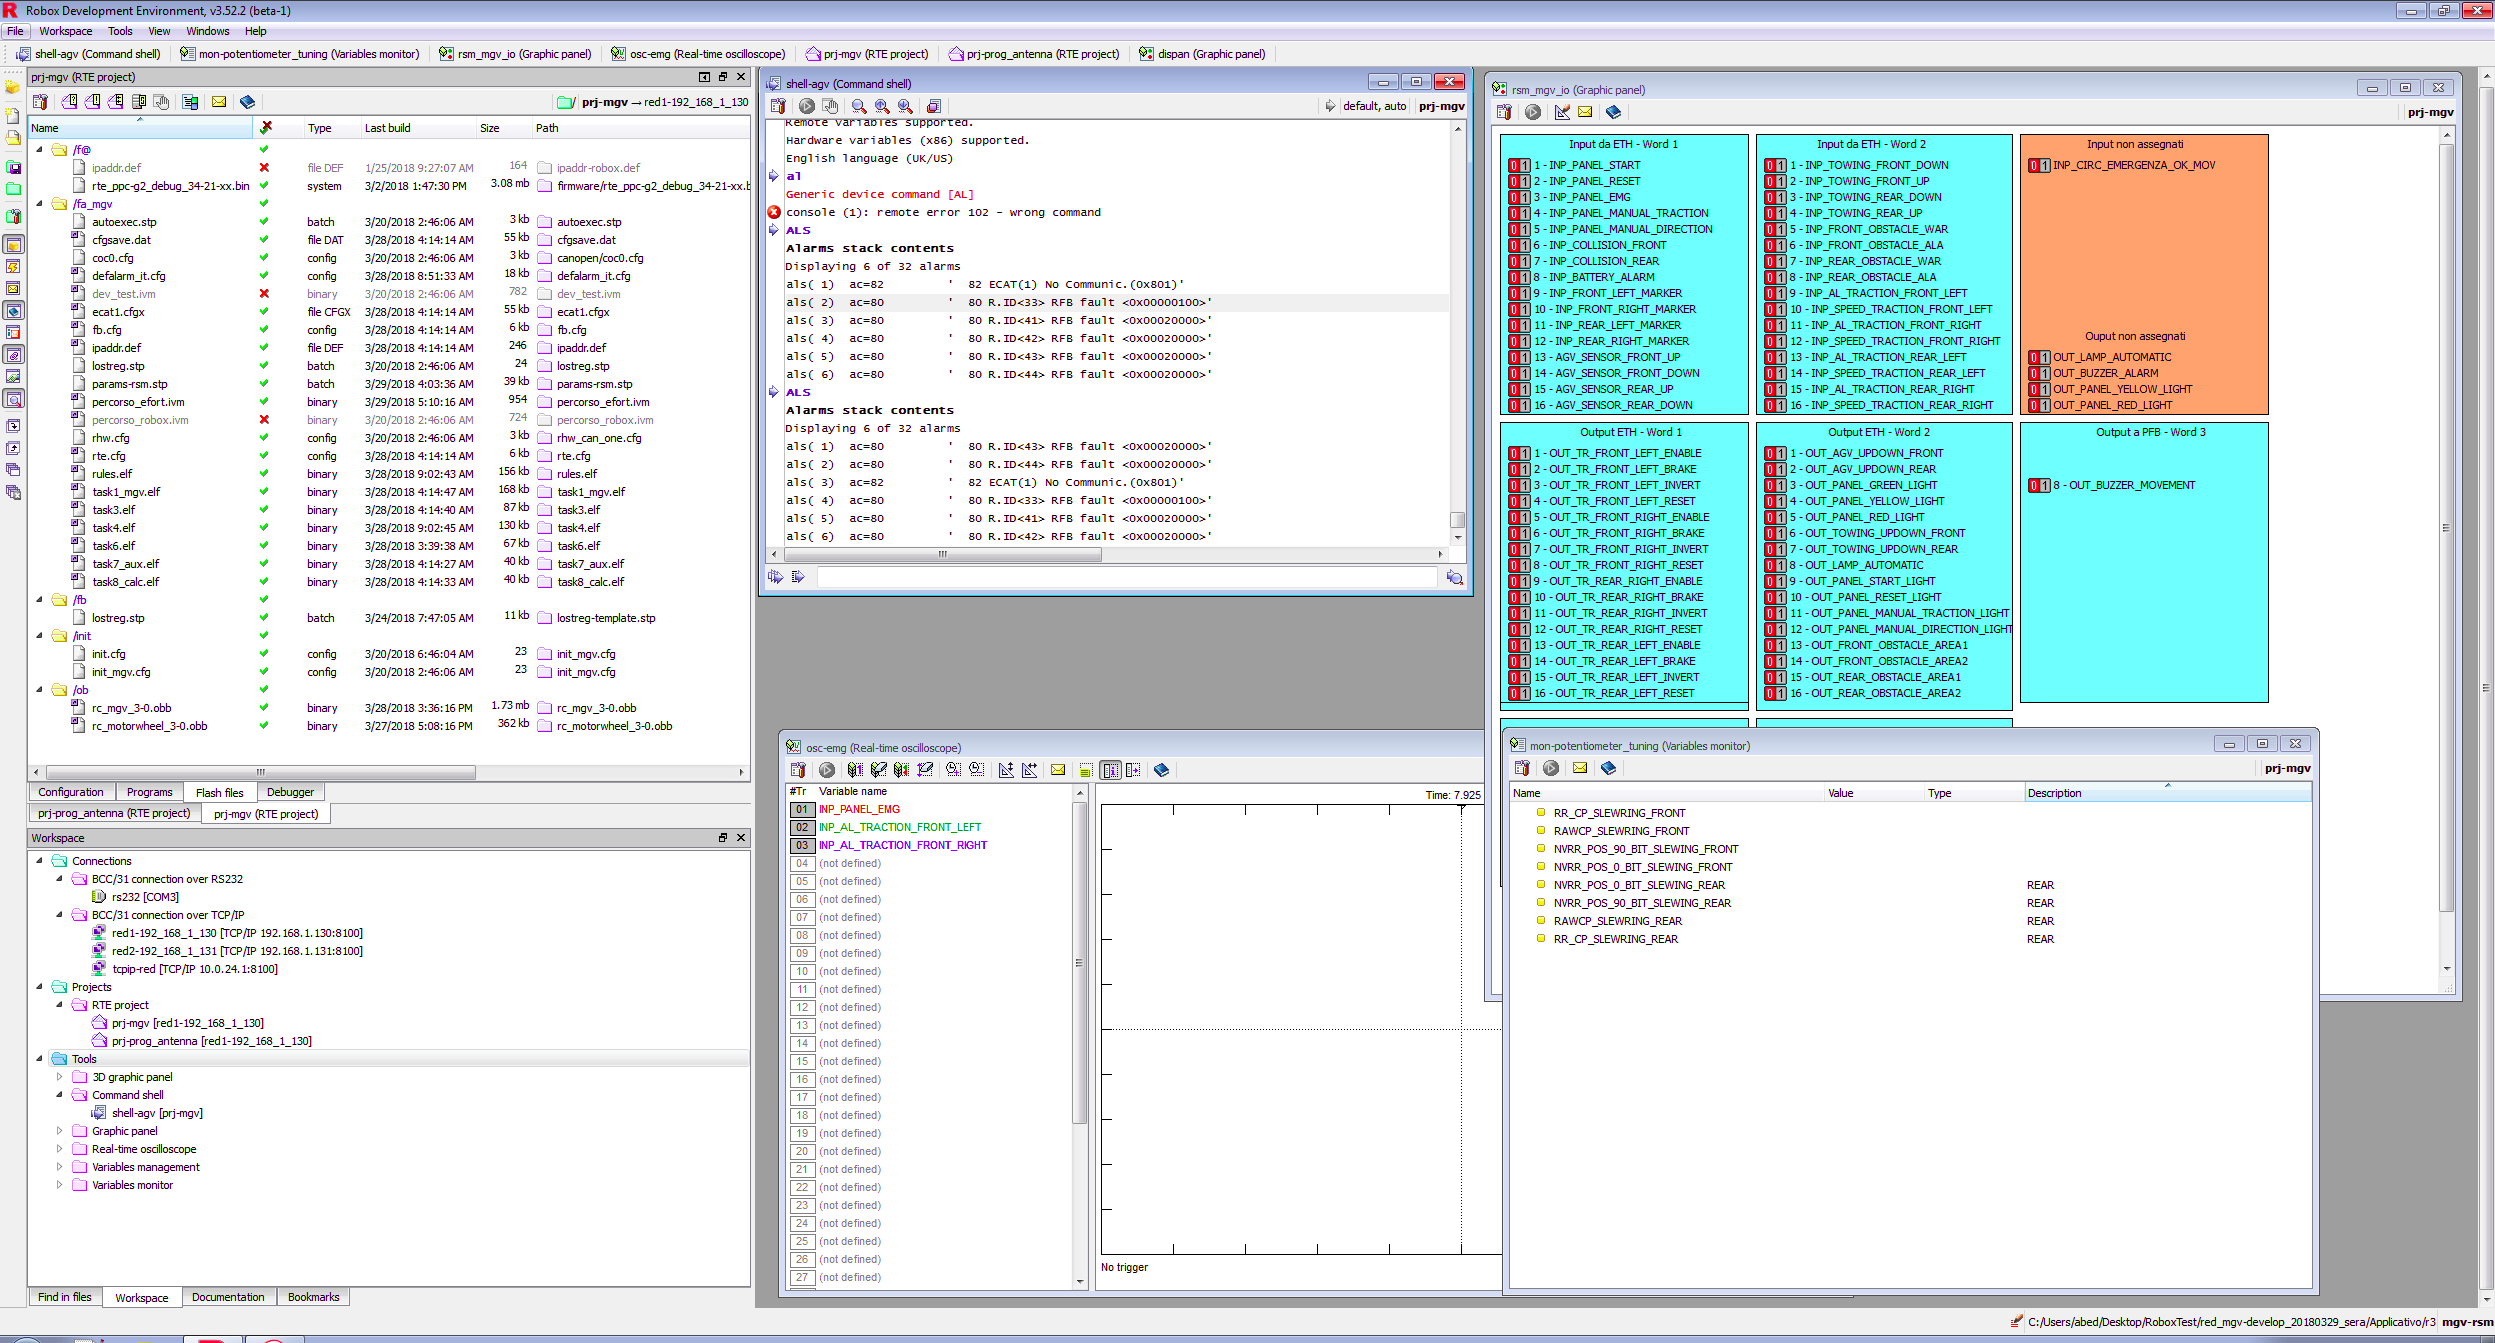
\includegraphics[scale=0.25, , angle =90]{rde/rde/rde1}
	\caption{RDE main windows}
	\label{figrde1}
\end{figure}

\section{First step}
In order to getting started with the controller, we need a memory card where we have to copy RTE and some configuration file. A new memory card will have the folder KEY that is generated by Robox for license.

After the installation of RDE, RCE and Icmap we need to copy in the installation folder the license in order to compile programs. The license is provided by Robox.

Before creating a new project, a workspace have to be created. A workspace may contain more than one project. In the menu bar, the workspace menu, allow to open, create and manage workspaces, also to access the predefined examples .

%----------------------------------------------------------------------------------------
%	 
%----------------------------------------------------------------------------------------
\section{New RTE project}

%----------------------------------------------------------------------------------------
%	 Tools
%----------------------------------------------------------------------------------------
\section{Tools}
From the workspace we can access the tools provided by RDE. Different king of tools are provided to debug and monitor the software: panels, oscilloscope, variable monitors and command shell.

\begin{figure}
	\centering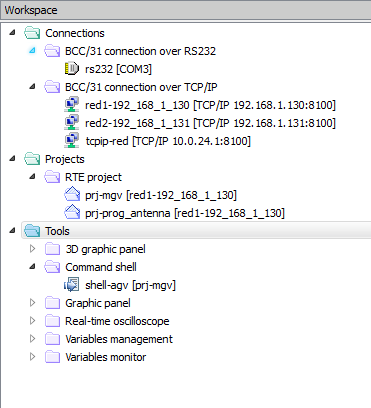
\includegraphics[scale=0.8]{rde/rde/workspace}
	\caption{Workspace}
	\label{figtools}
\end{figure}

%------------------
%	Command shell
%------------------
\subsection{Command shell}
The shell allow to interact with the controller via shell commands and device commands.
The most important commands for debugging are \textcolor{red}{sysinfo} to get information about the controller, \textcolor{red}{als} to get the list of alarms in the stack and \textcolor{red}{mreport} to get a report about the activities of the controller, the result is a log menu that can be exported to text file..

We can make shortcuts to the most used commands. Click the mouse right button and go to \textcolor{blue}{set quick commands} in order to define shortcuts. A list of defined shortcuts is available from the function keys [F1-F12] and from the action menu accessible from the mouse right click.

\begin{figure}
	\centering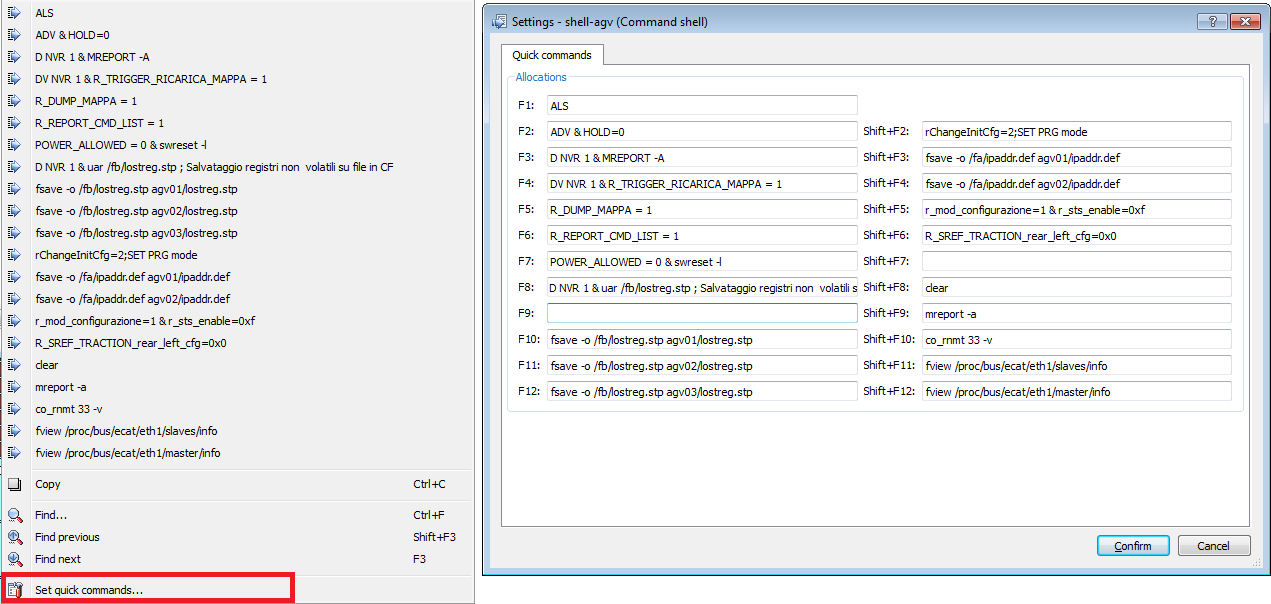
\includegraphics[scale=0.5 , angle =90]{rde/rde/quickcommands}
	\caption{Command shell: Quick commands}
	\label{figquickcommands}
\end{figure}

There are different types of commands, some types to manage variables others to manage the flash card other the device. A list of commands is available in the official documentation.

We will see some of the most used commands divided by category. Several commands can be used alone or with options. More than one command can be sent together by using the \textcolor{red}{\&} operator. Take a look at fig.\ref{figquickcommands} in order to see the usage and syntax of some commands.

\subsubsection{Variable management}
\textcolor{blue}{DV}: Display variable value. The dv command allow us to monitor the value of variables e.g. \textcolor{red}{dv nvr 1} display the value of the register \textcolor{red}{nvr(1)}.

\textcolor{blue}{SV}: Set variable value

\textcolor{blue}{FV}: Force variable value

\textcolor{blue}{RV}: Release variable value

\subsubsection{Device management}
\textcolor{blue}{adv}: Resets the device alarm

\textcolor{blue}{sysinfo}: Get information on connected device.

\textcolor{blue}{mreport}: It displays the events log. the option \textcolor{red}{-a} display all reports. Other options are available in order to filter the report.

\textcolor{blue}{als}: It displays the contents of the alarms stack.

\textcolor{blue}{swreset}: Request for software reset.

\textcolor{blue}{uar}: Opens a file present in the flash card and refreshes the assignments to  R, NVR, RR, NVRR, SR and NVSR with the current values but leaves the comment lines unchanged.

\subsubsection{Flash management}
\textcolor{blue}{fsave}: Save file from flash.

\textcolor{blue}{fview}

\subsubsection{Example of use}

\begin{description}
	\item[nvr 1 5] Set the value of nvr register 1 to 5, equivalent to \textcolor{blue}{sv nvr 1 5}
	\item[nvr 4.2 1] Set the bit 2 of nvr register 4 to 1
	\item[d inp\_w 100]
	\item[d inp 1]
	\item[d nvr 1]
	\item [d nvr 2.3]
	\item [d nvr 1 5] Displays 5 registers starting from 1
	\item [d nvr 1 5 -v]  Displays 5 registers starting from 1 with their index
	\item[f\_inp 300] Force logical state of input 300
	\item[uar /fb/lostreg.stp] Save the value of register in the file lostreg.stp
\end{description}

%------------------
%	
%------------------
\subsection{Oscilloscope}


%------------------
%	
%------------------
\subsection{Graphic panel}


%----------------------------------------------------------------------------------------
%	 
%----------------------------------------------------------------------------------------
\section{Hardware configuration}

%------------------
%	
%------------------
\subsection{Important folders and files}
Add new folder fig.\ref{fig:newfolder}

\begin{figure}[h]
	\centering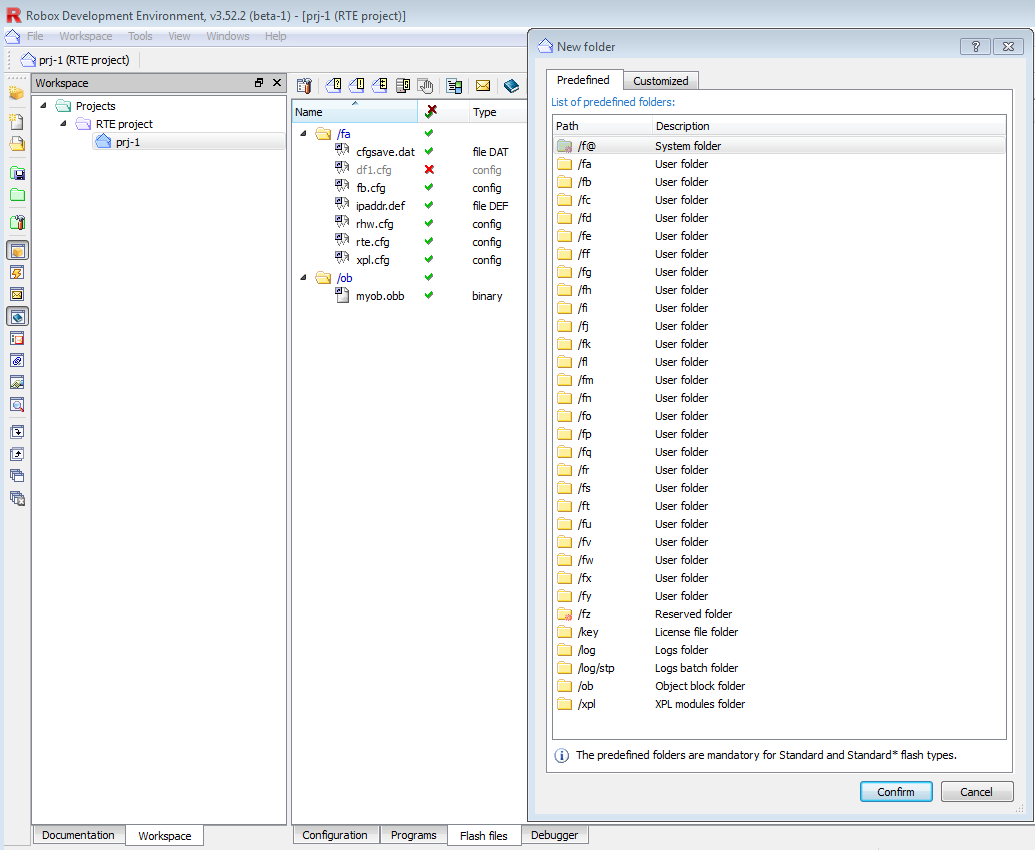
\includegraphics[scale=0.5]{rde/rde/newfolder}
	\caption{Add new folder to flash memory}
	\label{fig:newfolder}
\end{figure}

rte-xxxx.bin

rte.cg

ipaddr.def

rhw.cfg

lostreg.stp

init.cfg

defalarm\_it.cfg

%------------------
%	
%------------------
\subsection{Registers}

fig.\ref{fig:general-storage} show different types of registers and their allocation in memory.

\begin{figure}[h]
	\centering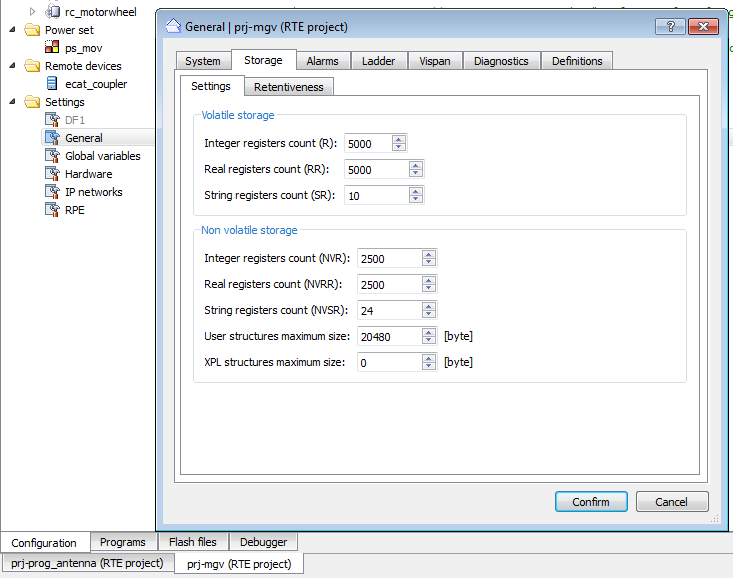
\includegraphics[scale=0.8]{rde/rde/general-storage}
	\caption{Register dimension}
	\label{fig:general-storage}
\end{figure}

%------------------
%	
%------------------
\subsection{Bus configuration}

%------------------
%	
%------------------
\subsection{Axes configuration}

%----------------------------------------------------------------------------------------
%	 
%----------------------------------------------------------------------------------------
\section{Programming languages}

%------------------
%	
%------------------
\subsection{R3}

%------------------
%	
%------------------
\subsection{Object block}
Object block is a C++ class, it is another option to write program in RDE. It is composed from a header file and a source file like like any C++ class, in addition to these classic files, RDE use the obs file to describe the interface of the Object block.

In rte project, right click and add new Object block fig.\ref{fig:obnew}. A folder have to be selected for the complied file. If the folder ob dosen't exist add it in the flash memory, see section files and folders.

\begin{figure}[h]
	\centering
	\begin{subfigure}{0.6\textwidth}
		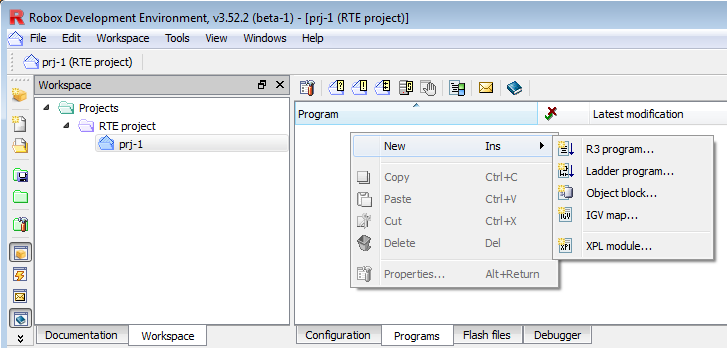
\includegraphics[width=\textwidth]{rde/rde/ob-new}
		\caption{Create new Object block. right click in the tab program of an RTE project}
		\label{fig:ob-new}
	\end{subfigure}
	\quad
	\begin{subfigure}{0.4\textwidth}
		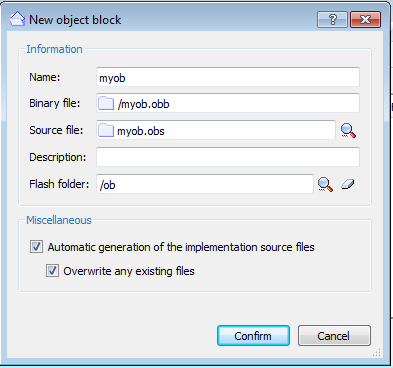
\includegraphics[width=\textwidth]{rde/rde/ob-new2}
		\caption{Write the OB name, select the folder of destination and check at least the first option.}
		\label{fig:ob-new2}
	\end{subfigure}
	\begin{subfigure}{0.4\textwidth}
		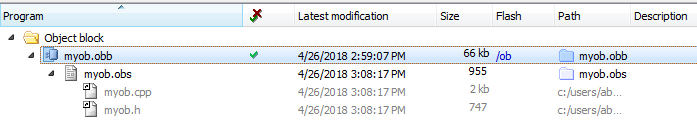
\includegraphics[width=\textwidth]{rde/rde/ob-new3}
		\caption{Object block structure files}
		\label{fig:ob-new3}
	\end{subfigure}
	\caption{New object block}
	\label{fig:obnew}
\end{figure}

After the creation of a new object block we will obtain 4 files:
\begin{enumerate}
	\item obs : object block interface file
	\item h : C++ header
	\item cpp : C++ source
	\item obb : Object block binary file (compiled file)
\end{enumerate}

Fig.\ref{fig:obobs}, \ref{fig:obheader} and \ref{fig:obcpp} show the auto generated files. As we can see the header and the source files have the structure of a classic C++ class with class name, class constructor and destructor.
\begin{figure}[h]
	\centering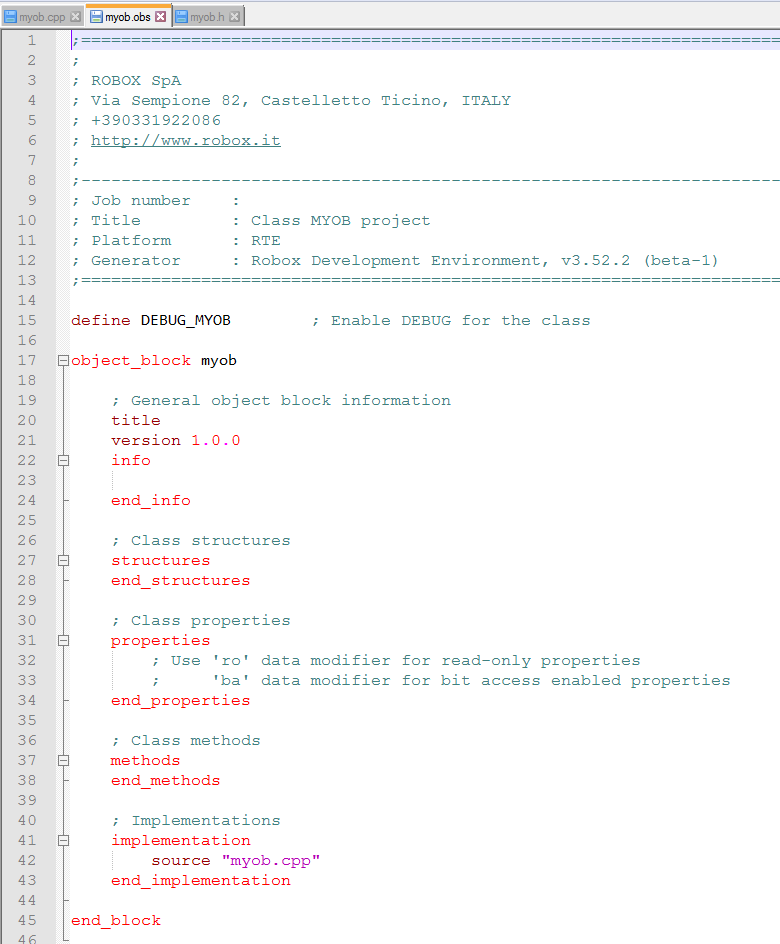
\includegraphics[scale=0.5]{rde/rde/obobs}
	\caption{Auto-generated OBS file}
	\label{fig:obobs}
\end{figure}

\begin{figure}[h]
	\centering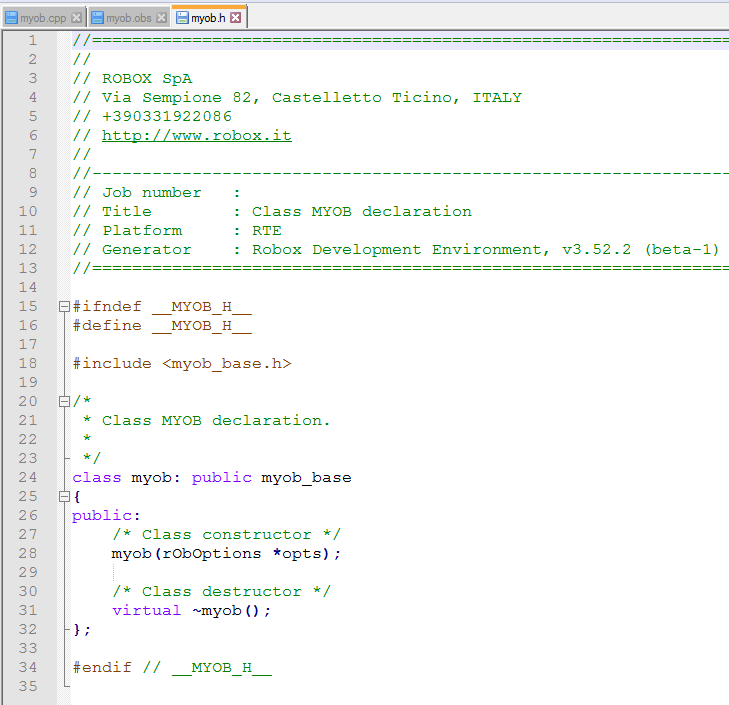
\includegraphics[scale=0.5]{rde/rde/obheader}
	\caption{Auto-generated C++ header}
	\label{fig:obheader}
\end{figure}

\begin{figure}[h]
	\centering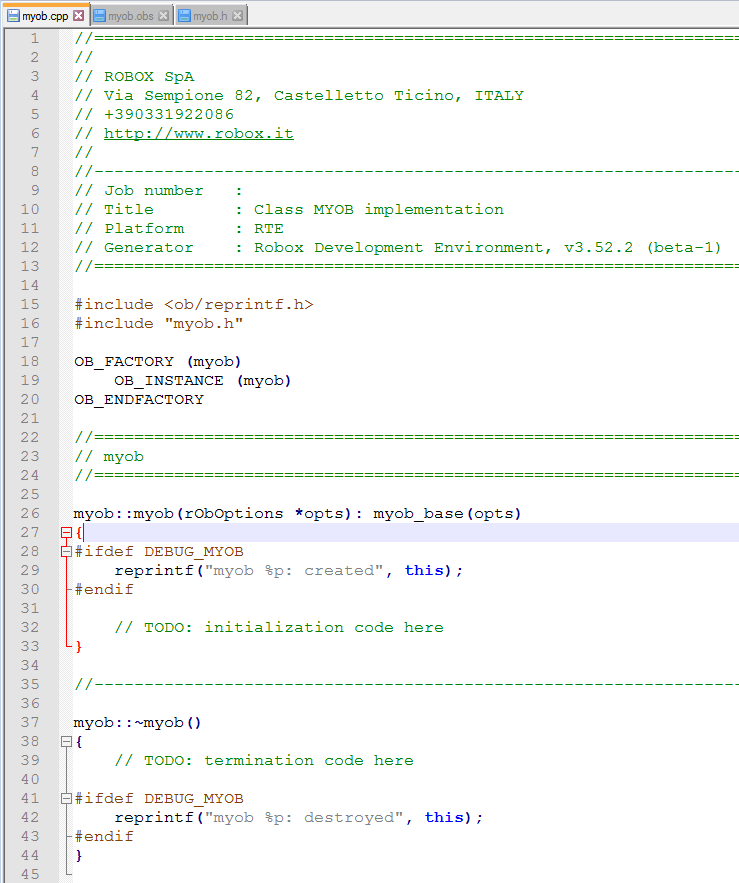
\includegraphics[scale=0.5]{rde/rde/obcpp}
	\caption{Auto-generated C++ source}
	\label{fig:obcpp}
\end{figure}

As any class of an object oriented language, an Object block have methods (functions) and fields (variables). Public methods and fields that can be accessed from an R3 program should be written in the obs file respectively in the methods and properties blocks.
Properties could be only of simple C++ types: BOOL, I8, I16, I32, U8, U16, U32, INT, FLOAT, REAL, CHAR,could not be of struct type.
The source file where the code is implemented is written in the block implementation. Fig.\ref{fig:obsex} show an example of an obs file.

\begin{figure}[h]
	\centering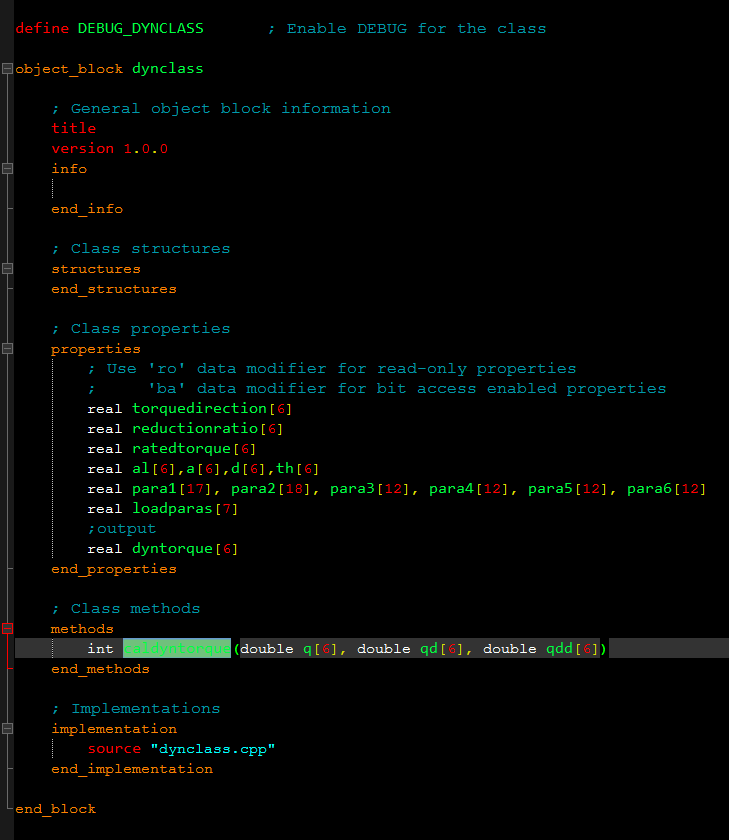
\includegraphics[scale=0.5]{rde/rde/obs-example}
	\caption{Obs example file}
	\label{fig:obsex}
\end{figure}

As any object oreinted language, a class have to be instantiated before using it. In the configuration tab of an RTE project, right click Object block and add OB class or OB instance, fig.\ref{fig:obclass}. A class could have more than one instance. An OB is similar to an FB (Function block) in PLc programming.

\begin{figure}[h]
	\centering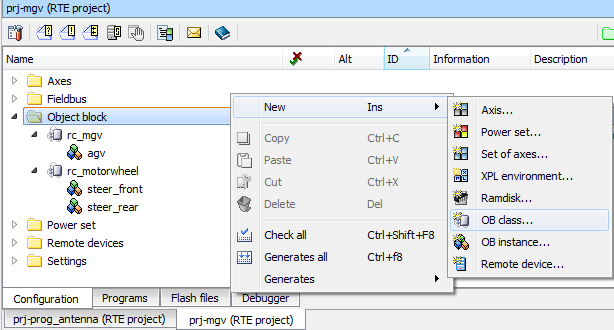
\includegraphics[scale=0.6]{rde/rde/ob-class}
	\caption{OB Class or instance. Add a class than add an instance. In the figure we can see 2 classes : rc\_mgv and rc\_motorwheel, and one instance of the first class and two instances of the second one.}
	\label{fig:obclass}
\end{figure}

\begin{figure}[h]
	\centering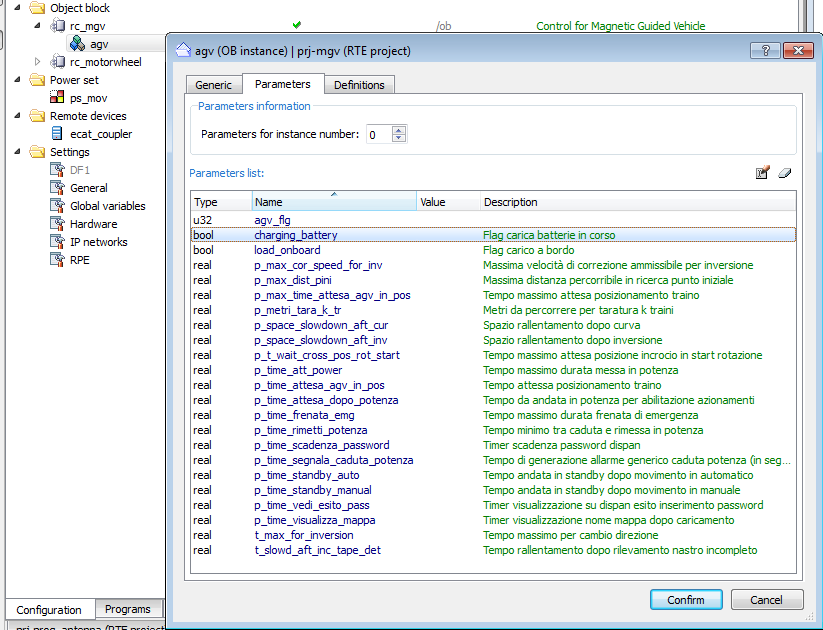
\includegraphics[scale=0.6]{rde/rde/ob-instancepar}
	\caption{Object block instance parameters. In the column \textcolor{blue}{Value} we can initialize the variables. To keep the program easy to read, it is better to initialize OB properties in R3. Note that properties declared as \textcolor{blue}{ro} (read-only) are not shown here}
	\label{fig:obinstancepar}
\end{figure}

Suppose we have the class \textcolor{blue}{rc\_mgv} and its instance \textcolor{blue}{agv}, as in fig.\ref{fig:obclass}. We can call in R3 the method \textcolor{blue}{get\_status} of the class \textcolor{blue}{rc\_mgv} as we call it in C++: \textcolor{red}{agv.get\_status(AgvStatus\_t4)}. We can access properties using also the dot operator for reading or writing: \textcolor{red}{agv.DRIVING\_MODE\_TAPE = 4} or \textcolor{red}{if(agv.TAPE\_FOLLOW\_LEFT)}.

If we defined a structure in the obs file we can use it to define a variable of that type in R3 using the dot operator.

%------------------
%	
%------------------
\subsubsection{OB Predefined example}
In menu file, workspace, specials, predefined examples, we can find the example OB: Use and OB implementation. This example provide the source code an OB, rc\_belt, that handle a belt and a rules and task 1 implementation.
The Class rc\_belt is an OB that can be find in the Object Block library. The example use another OB from the standard library, rc\_axis, without providing its source code.

Refer to the official Object Block documentation for more informations about OB classes.

\begin{figure}[h]
	\centering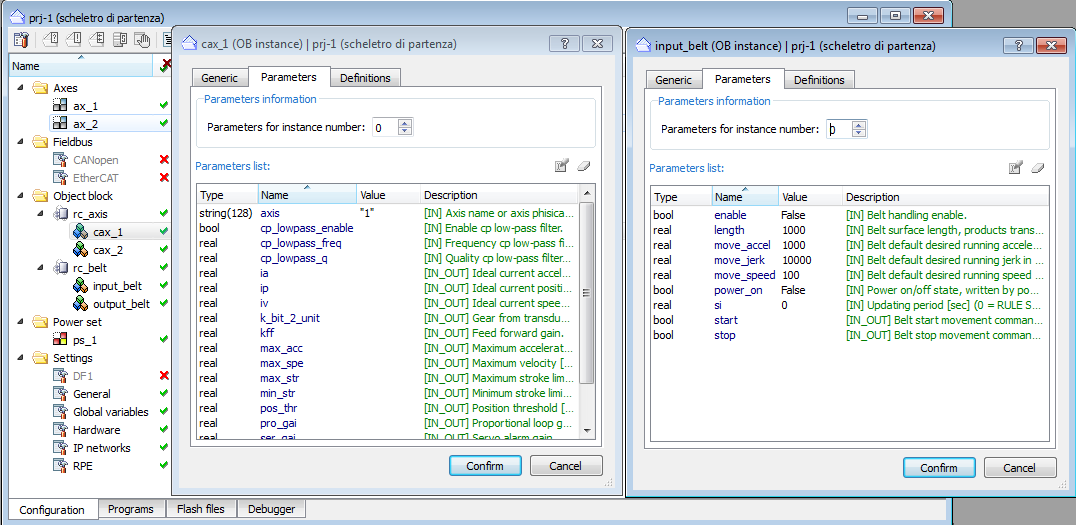
\includegraphics[scale=0.6]{rde/rde/ob-belt-example}
	\caption{OB: Use and OB implementation predefined example.}
	\label{fig:obbeltexample}
\end{figure}

In the obs file of rc\_belt, we can see the interface of the Class, how to use another class by importing it, define inputs and outputs and some methods. Note that input and outputs deffer only with the keyword \textcolor{red}{ro}. When an property is declared as read only behave like an output, otherwise behave like an input.

In the implementation we can see the call to two C++ source files. In this OB, 2 classes were defined. The class rc\_belt, that inherit from rc\_belt\_base, and the class RCBelt.\\

A detailed example about OB implementation will be provided in the chapter related to motion control.

%----------------------------------------------------------------------------------------
%	   Programs
%----------------------------------------------------------------------------------------
\section{Programs}

%------------------
%	
%------------------
\subsection{Tasks}

%------------------
%	
%------------------
\subsection{Rules}

%------------------
%	
%------------------
\subsection{R3 example program}

%------------------
%	
%------------------
\subsection{OB example program}


%----------------------------------------------------------------------------------------
%	 Axis control example
%----------------------------------------------------------------------------------------
\section{Axis control example}

%------------------
%	
%------------------
\subsection{Axis configuration}

%------------------
%	
%------------------
\subsection{Power set and power handling}

%------------------
%	
%------------------
\subsection{Velocity control}

%------------------
%	
%------------------
\subsection{Position control}




